En la sexta clase del curso, trabajaremos con algor\'itmos de clasificaci\'on  supervisados. Son nuestros objetivos:

\begin{itemize}
  \item Poder realizar clasificaciones supervisadas utilizando los distintos algor\'itmos que se encuentran en R.
  \item Comparar, utilizando la entrop\'ia de un p\'ixel, que coberturas presentan  mayor confusi\'on al momento de la clasificaci\'on.
\end{itemize}

Cargaremos primero la imagen Landsat 8 y habilitaremos la opci\'on para escribir el header de ENVI\@. Usaremos en primer lugar los paquetes \texttt{raster}, \texttt{rgdal}, \texttt{RStoolbox} y \texttt{rasterVis}.

\begin{lstlisting}
    rasterOptions(addheader = "ENVI")
    xml.2016 <- readMeta("raster_data/LC82240782016304/LC82240782016304LGN00.xml")
    ref.2016 <- stackMeta(xml.2016, quantity = "sre")
    scaleF <- getMeta(ref.2016,xml.2016, what = "SCALE_FACTOR")
    ref.2016 <- ref.2016 * scaleF
    ref.2016 <- ref.2016[[-1,]]
    names(ref.2016) <- c("blue","green","red","nir","swir1","swir2")
    vector <- readOGR(dsn="vector_data", layer="entrenamiento")
\end{lstlisting}

\section{Clasificaci\'on por m\'axima verosimilitud}

Empecemos con la clasificaci\'on por el m\'etodo de m\'axima verosimilitud (figura \ref{fig:MC}).

\begin{lstlisting}
    library(e1071)
    colores = c('#b2df8a','#33a02c',
                '#fdbf6f','#ff7f00',
                '#fb9a99','#e31a1c',
                '#a6cee3','#1f78b4')
    sup.2016 <- superClass(ref.2016, vector, responseCol = "MC_ID",
                           model = "mlc")
    plot(sup.2016$map, col=colores, zlim=c(1,8))
\end{lstlisting}

\begin{figure}[h!]
  \centering
  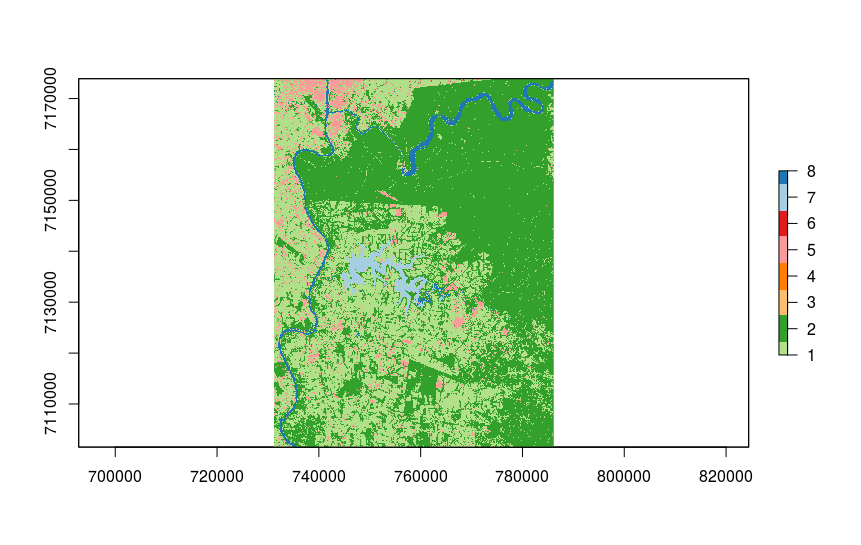
\includegraphics[width=0.7\textwidth]{mlc-MC.png}
  \caption{Clasificaci\'on por m\'axima verosimilitud sin separar en clases espectrales.}
  \label{fig:MC}
\end{figure}

Cambiando el algor\'itmo de clasificaci\'on en el par\'ametro \texttt{model} podemos calcular distintas clasificaciones supervisadas. Algunas de las vistas en clase son \texttt{mlc}, \texttt{rf} y \texttt{svmRadial}. Cada una de ellas usa alguna libreria adicional.

\begin{exa}
  Una forma de mejorar las clasificaciones supervisadas es clasificar por separado distintas clases espectrales y luego unirlas en la misma clase de informaci\'on. Veamos como hacerlo.

  \begin{lstlisting}
      sup.2016b <- superClass(ref.2016, vector, responseCol = "C_ID",
                             model = "mlc")
  \end{lstlisting}

  En este caso, la columna de respuestaa es \texttt{C\_ID} y no \texttt{MC\_ID}.  Una vez realizada la clasificaci\'on, debemos substituir los valores de cada p\'ixel por el de la clase de informaci\'on correspondiente. Para ello:

  \begin{lstlisting}
    subs.2016 = vector@data[c(3,1)]
    sub.2016 <- reclassify(sup.2016b$map, subs.2016)
    writeRaster(sub.2016, "raster_data/processed/mlc2016",
                datatype="INT1U")
  \end{lstlisting}

    Podemos finalmente comparar las dos imagenes clasificadas lado a lado ejecuntado el comando \verb|plot(stack(sup.2016$map,sub.2016),col=colores,zlim=c(1,8))| (figura \ref{fig:mlc}).

    \begin{figure}[h!]
      \centering
      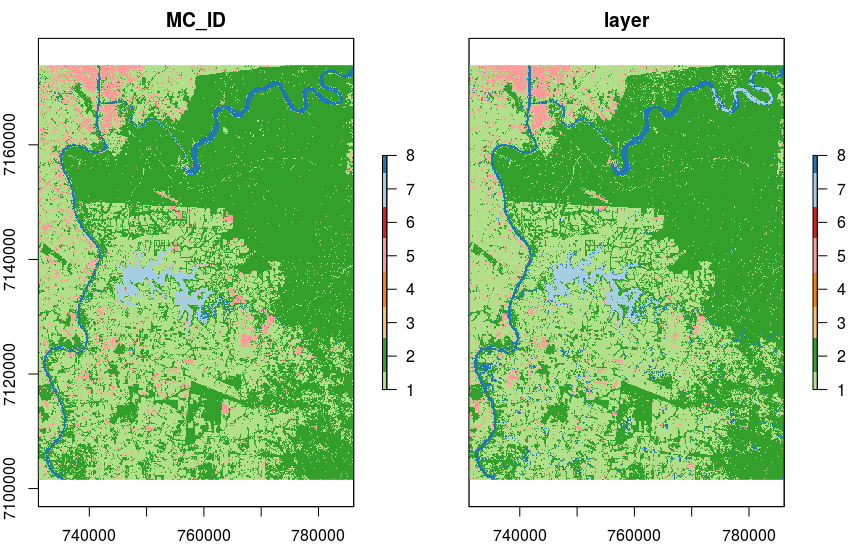
\includegraphics[width=0.7\textwidth]{mlc-comparacion.png}
      \caption{Comparaci\'on entre la clasificaci\'on utilizando clases de informaci\'on y clases espectrales.}
      \label{fig:mlc}
    \end{figure}
\end{exa}

\begin{act}
    Realice clasificaciones por los distintos m\'etodos y comparelas visualmente.
\end{act}

\begin{act}
    Agregue las bandas de textura y vuelva a clasificar las im\'agenes.
\end{act}

\section{Entrop\'ia de la clasificaci\'on}

Para poder comparar en que zonas los clasificadores presentan mas o menos dispersi\'on podemos calcular la entrop\'ia de las distintas clasificaciones en cada p\'ixel. Para esto utilizaremos la funcion \texttt{rasterEntropy}.

\begin{exa}
  Comenzamos corriendo la clasificaci\'on para distintos modelos.

  \begin{lstlisting}
      set.seed(42)
      library(e1071)
      sup.2016 <- superClass(ref.2016, vector, responseCol = "C_ID",
                           model = "mlc")
      mlc.2016 <- reclassify(sup.2016$map, subs.2016)

      library(randomForest)
      sup.2016 <- superClass(ref.2016, vector, responseCol = "C_ID",
                           model = "rf")
      rf.2016 <- reclassify(sup.2016$map, subs.2016)

      library(kernlab)
      sup.2016 <- superClass(ref.2016, vector, responseCol = "C_ID",
                           model = "svmLinear")
      svm.2016 <- reclassify(sup.2016$map, subs.2016)
  \end{lstlisting}

  Los apilamos y calculamos la entrop\'ia en cada p\'ixel.

  \begin{lstlisting}
      prediction_stack <- stack(mlc.2016, rf.2016, svm.2016)
      names(prediction_stack) <- c("mlc","rf","svm")
      model_entropy <- rasterEntropy(prediction_stack)
  \end{lstlisting}

  Podemos graficar la entrop\'ia de las clasificaciones como \verb|model_entropy| y ver que zonas presentan mayor o menor diferencia, a la hora de la clasificacion (figura \ref{fig:entropia}).

  \begin{lstlisting}
    plot(stack(prediction_stack, model_entropy),col=colores)
  \end{lstlisting}

  \begin{figure}[h!]
    \centering
    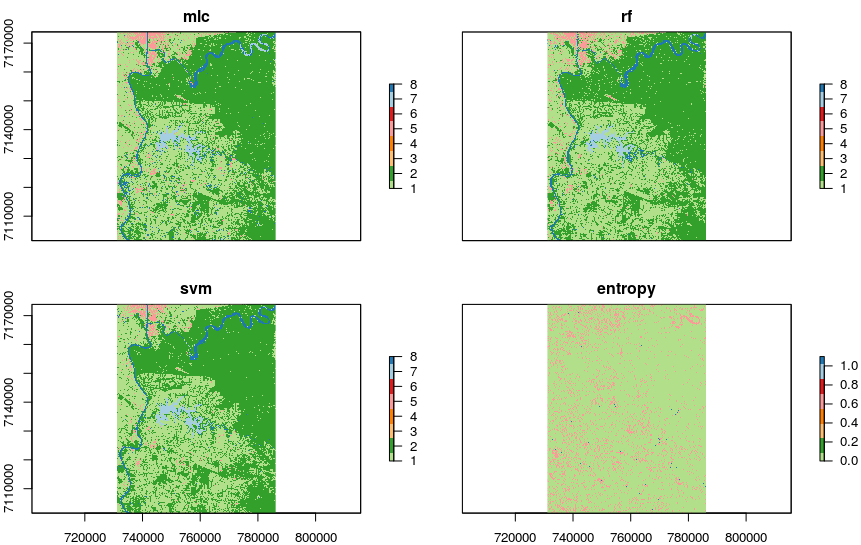
\includegraphics[width=0.6\textwidth]{comparacion-sup.png}
    \caption{Comparaci\'on entre los distintos m\'etodos de clasificaci\'on supervisada usando la entrop\'ia de la clasificaci\'on.}
    \label{fig:entropia}
  \end{figure}

\end{exa}

\begin{act}
  Repita las clasificaciones por los m\'etodos de arriba agregando (maxima verosimilitud, random forest, support vector machine) la banda textura. Apilela junto con las clasificaciones por k-means de la clase anterior. ¿A que cobertura pertenecen las zonas con mayor variabilidad?
\end{act}
